% !TEX TS-program = pdflatex
\documentclass[11pt]{article}

% -------------------- Packages --------------------
\usepackage[a4paper,margin=1in]{geometry}
\usepackage{amsmath,amssymb}
\usepackage[T1]{fontenc}
\usepackage{lmodern}
\usepackage{xcolor}
\usepackage{tcolorbox}
\tcbuselibrary{skins,breakable}
\usepackage{enumitem}
\usepackage{hyperref}
\usepackage{tikz}
\usetikzlibrary{calc,angles,quotes,arrows.meta}

\pagestyle{empty}

% -------------------- Dark Theme Colors --------------------
\definecolor{bg}{HTML}{000000}
\definecolor{pairbg}{HTML}{121212}
\definecolor{solbg}{HTML}{0A0A0A}
\definecolor{border}{HTML}{2A2A2A}
\definecolor{text}{HTML}{FFFFFF}
\definecolor{muted}{HTML}{C9CDD3}
\definecolor{gold}{HTML}{FFD700}
\definecolor{green}{HTML}{4ADE80}
\definecolor{cyan}{HTML}{38BDF8}

\pagecolor{bg}
\color{text}

\hypersetup{
  colorlinks=true,
  linkcolor=cyan,
  urlcolor=cyan
}

\setlength{\parindent}{0pt}
\setlength{\parskip}{10pt}

% Help LaTeX avoid overfull lines globally
\sloppy
\setlength{\emergencystretch}{3em}

\setlist[itemize]{left=1.4em,itemsep=6pt,topsep=6pt}
\setlist[enumerate]{left=1.6em,itemsep=4pt,topsep=4pt}

% -------------------- tcolorbox Base --------------------
\tcbset{
  enhanced,
  breakable,
  arc=12pt,
  boxrule=0.8pt,
  left=14pt,right=14pt,top=12pt,bottom=12pt
}

\newtcolorbox{QAPair}[1]{%
  colback=pairbg,
  colbacklower=solbg,
  colframe=border,
  coltext=text,
  title=\textcolor{gold}{\bfseries #1},
  fonttitle=\bfseries,
  coltitle=text,
  segmentation style={draw=border, dashed, line width=0.6pt},
  before upper=\raggedright,
  before lower=\raggedright
}

\newtcolorbox{QuickBox}{%
  colback=pairbg,
  colframe=cyan,
  coltext=text,
  fontupper=\color{text}\raggedright,
  borderline north={4pt}{0pt}{cyan},
  arc=14pt,
  boxrule=0.8pt
}

% Helper for step headings
\newcommand{\Step}[1]{\textcolor{muted}{\textbf{Step #1:}}}

% Small centered diagram block
\newenvironment{StepDiagram}{\par\medskip\begin{center}}{\end{center}\medskip}

% TikZ styles
\tikzset{
  base/.style={draw=text, line width=0.9pt, line cap=round, line join=round},
  new/.style={draw=cyan, line width=1.2pt, line cap=round, line join=round},
  help/.style={draw=muted, dashed, line width=0.9pt},
  ang/.style={draw=gold, line width=1.0pt},
  dot/.style={circle, fill=text, inner sep=1.2pt},
  lab/.style={text=text, font=\small},
  labm/.style={text=muted, font=\small},
  tag/.style={fill=pairbg, inner sep=1.5pt, rounded corners=2pt, text=text, font=\small},
}

\newcommand{\EqDiagram}[1]{%
\begin{StepDiagram}
\begin{tikzpicture}
\node[draw=border, rounded corners=10pt, inner sep=8pt, text=text, align=left, text width=0.85\linewidth] {#1};
\end{tikzpicture}
\end{StepDiagram}
}

% Small helper for consistent circle sketches (no clutter)
\newcommand{\MiniCircle}[2]{% radius, extra drawings
\begin{tikzpicture}[scale=0.92]
  \def\r{#1}
  \coordinate (O) at (0,0);
  \draw[base] (O) circle (\r);
  #2
\end{tikzpicture}
}

% ============================================================
\begin{document}

\begin{center}
{\LARGE\bfseries \textcolor{gold}{Exercise 11.1 --- Constructions \& Solutions}}\\[-2pt]
\end{center}

% -------------------- Quick ideas + small diagrams --------------------
\begin{QuickBox}
{\color{cyan}\bfseries Quick ideas (How to find a circle/centre)}\par\medskip

\begin{itemize}
\item \textbf{Centre of a circle:} The perpendicular bisector of any chord passes through the centre.  
So draw \emph{two} chords and their perpendicular bisectors; their intersection is the centre.
\begin{StepDiagram}
\MiniCircle{2.1}{
  \coordinate (A) at (-1.6,0.8);
  \coordinate (B) at ( 1.6,0.8);
  \coordinate (C) at (-1.2,-0.4);
  \coordinate (D) at ( 1.2,1.6);
  \coordinate (M1) at ($(A)!0.5!(B)$);
  \coordinate (M2) at ($(C)!0.5!(D)$);

  \draw[new] (A)--(B);
  \draw[new] (C)--(D);

  \draw[help] ($(M1)+(0,-1.7)$) -- ($(M1)+(0,1.7)$);
  \draw[help] ($(M2)+(-1.7,0)$) -- ($(M2)+(1.7,0)$);

  \node[dot] at (O) {};
  \node[tag] at ($(O)+(0.35,-0.25)$) {$O$};
  \node[labm] at (0,-2.55) {Intersection of two bisectors = centre};
}
\end{StepDiagram}

\item \textbf{Circle through three points:} For non-collinear points $A,B,C$, the centre is the intersection of the perpendicular bisectors of $AB$ and $BC$. This centre is the \textbf{circumcentre}.
\begin{StepDiagram}
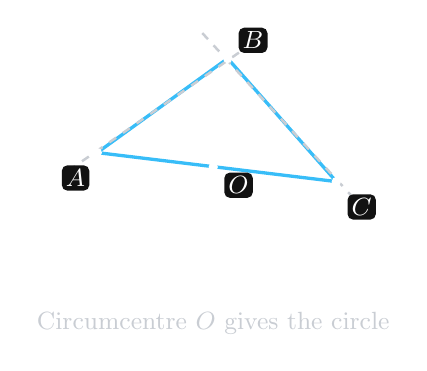
\begin{tikzpicture}[scale=0.92]
  \coordinate (A) at (-1.6,0.2);
  \coordinate (B) at ( 0.2,1.5);
  \coordinate (C) at ( 1.7,-0.2);
  \coordinate (M1) at ($(A)!0.5!(B)$);
  \coordinate (M2) at ($(B)!0.5!(C)$);
  \coordinate (O) at (0,0);

  \draw[new] (A)--(B)--(C)--cycle;

  \draw[help] ($(M1)+(-1.3,-0.9)$) -- ($(M1)+(1.3,0.9)$);
  \draw[help] ($(M2)+(-1.1,1.2)$) -- ($(M2)+(1.1,-1.2)$);

  \node[dot] at (A) {}; \node[tag] at ($(A)+(-0.3,-0.35)$) {$A$};
  \node[dot] at (B) {}; \node[tag] at ($(B)+(0.35,0.25)$) {$B$};
  \node[dot] at (C) {}; \node[tag] at ($(C)+(0.35,-0.35)$) {$C$};

  \node[dot] at (O) {}; \node[tag] at ($(O)+(0.35,-0.25)$) {$O$};
  \node[labm] at (0,-2.15) {Circumcentre $O$ gives the circle};
\end{tikzpicture}
\end{StepDiagram}

\item \textbf{Right triangle trick:} In a right triangle, the circumcentre is the \textbf{midpoint of the hypotenuse}.  
So the circumradius $=\dfrac{\text{hypotenuse}}{2}$.
\begin{StepDiagram}
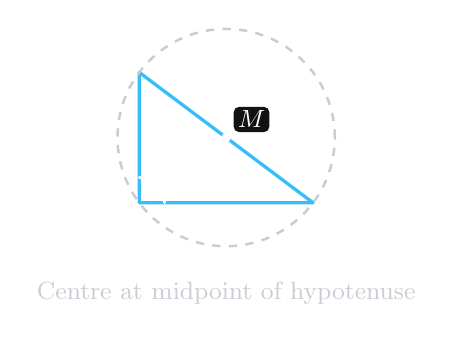
\begin{tikzpicture}[scale=0.92]
  \coordinate (Q) at (0,0);
  \coordinate (P) at (0,1.8);
  \coordinate (R) at (2.4,0);
  \coordinate (M) at ($(P)!0.5!(R)$);

  \draw[new] (P)--(Q)--(R)--cycle;
  \draw[base] ($(Q)+(0.35,0)$) -- ($(Q)+(0.35,0.35)$) -- ($(Q)+(0,0.35)$);

  \node[dot] at (M) {}; \node[tag] at ($(M)+(0.35,0.25)$) {$M$};
  \draw[help] (M) circle (1.5);
  \node[labm] at (1.2,-1.25) {Centre at midpoint of hypotenuse};
\end{tikzpicture}
\end{StepDiagram}

\item \textbf{Arc/circumference:} $C=2\pi r$. If each tile covers arc length $L$, then
\[
\text{Number of tiles}=\frac{2\pi r}{L}\quad(\text{round up}).
\]
\begin{StepDiagram}
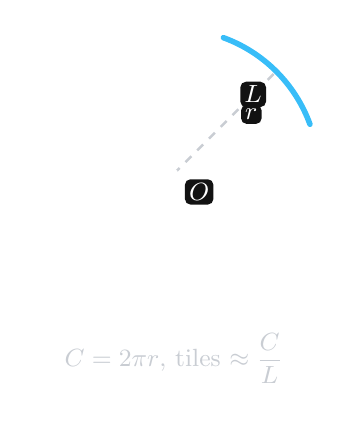
\begin{tikzpicture}[scale=0.92]
  \def\r{2.0}
  \coordinate (O) at (0,0);
  \draw[base] (O) circle (\r);
  \draw[new, line width=2pt] ({\r*cos(20)},{\r*sin(20)}) arc (20:70:\r);
  \draw[help] (O)--({\r*cos(45)},{\r*sin(45)});
  \node[tag] at ($(O)!0.58!({\r*cos(45)},{\r*sin(45)})+(0.25,0)$) {$r$};
  \node[tag] at ({1.55*cos(45)},{1.55*sin(45)}) {$L$};
  \node[dot] at (O) {};
  \node[tag] at ($(O)+(0.35,-0.25)$) {$O$};
  \node[labm] at (0,-2.55) {$C=2\pi r$, tiles $\approx \dfrac{C}{L}$};
\end{tikzpicture}
\end{StepDiagram}
\end{itemize}
\end{QuickBox}

% ============================================================
% Q1
\begin{QAPair}{Question 1}
\textcolor{gold}{\bfseries Question:} Given a circle, locate its centre.
\tcblower
\textcolor{green}{\bfseries Answer:}\par

\Step{1} Draw any chord $AB$ of the circle.
\begin{StepDiagram}
\MiniCircle{2.2}{
  \coordinate (A) at (-1.7,0.9);
  \coordinate (B) at ( 1.7,0.9);
  \draw[new] (A)--(B);
  \node[tag] at ($(A)+(-0.25,0.15)$) {$A$};
  \node[tag] at ($(B)+(0.25,0.15)$) {$B$};
}
\end{StepDiagram}

\Step{2} Construct the \textbf{perpendicular bisector} of chord $AB$.
\begin{StepDiagram}
\MiniCircle{2.2}{
  \coordinate (A) at (-1.7,0.9);
  \coordinate (B) at ( 1.7,0.9);
  \coordinate (M1) at ($(A)!0.5!(B)$);
  \draw[new] (A)--(B);
  \draw[help] ($(M1)+(0,-1.9)$) -- ($(M1)+(0,1.9)$);
  \node[tag] at ($(M1)+(0.35,0.0)$) {bisector};
}
\end{StepDiagram}

\Step{3} Draw another chord $CD$ (not parallel to $AB$).
\begin{StepDiagram}
\MiniCircle{2.2}{
  \coordinate (A) at (-1.7,0.9);
  \coordinate (B) at ( 1.7,0.9);
  \coordinate (C) at (-1.2,-0.5);
  \coordinate (D) at ( 1.3,1.6);
  \draw[new] (A)--(B);
  \draw[new] (C)--(D);
  \node[tag] at ($(C)+(-0.25,-0.25)$) {$C$};
  \node[tag] at ($(D)+(0.25,0.15)$) {$D$};
}
\end{StepDiagram}

\Step{4} Construct the perpendicular bisector of chord $CD$.
\begin{StepDiagram}
\MiniCircle{2.2}{
  \coordinate (A) at (-1.7,0.9);
  \coordinate (B) at ( 1.7,0.9);
  \coordinate (C) at (-1.2,-0.5);
  \coordinate (D) at ( 1.3,1.6);
  \coordinate (M1) at ($(A)!0.5!(B)$);
  \coordinate (M2) at ($(C)!0.5!(D)$);
  \draw[new] (A)--(B);
  \draw[new] (C)--(D);
  \draw[help] ($(M1)+(0,-1.9)$) -- ($(M1)+(0,1.9)$);
  \draw[help] ($(M2)+(-1.9,0)$) -- ($(M2)+(1.9,0)$);
}
\end{StepDiagram}

\Step{5} The two perpendicular bisectors intersect at the centre $O$.
\begin{StepDiagram}
\MiniCircle{2.2}{
  \coordinate (A) at (-1.7,0.9);
  \coordinate (B) at ( 1.7,0.9);
  \coordinate (C) at (-1.2,-0.5);
  \coordinate (D) at ( 1.3,1.6);
  \coordinate (M1) at ($(A)!0.5!(B)$);
  \coordinate (M2) at ($(C)!0.5!(D)$);
  \draw[new] (A)--(B);
  \draw[new] (C)--(D);
  \draw[help] ($(M1)+(0,-1.9)$) -- ($(M1)+(0,1.9)$);
  \draw[help] ($(M2)+(-1.9,0)$) -- ($(M2)+(1.9,0)$);
  \node[dot] at (O) {};
  \node[tag] at ($(O)+(0.35,-0.25)$) {$O$};
}
\end{StepDiagram}

\[
\boxed{\text{Centre }= \text{intersection of perpendicular bisectors of two chords.}}
\]
\end{QAPair}

% ============================================================
% Q2
\begin{QAPair}{Question 2}
\textcolor{gold}{\bfseries Question:} Three points $X$, $Y$ and $Z$ are located on an arc. Find the centre of that arc.
\tcblower
\textcolor{green}{\bfseries Answer:}\par

\Step{1} Join $XY$ and $YZ$ to make two chords.
\begin{StepDiagram}
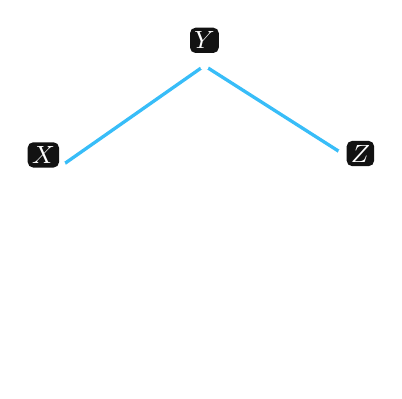
\begin{tikzpicture}[scale=0.92]
  \def\r{2.1}
  \coordinate (O) at (0,0);
  \coordinate (X) at ({\r*cos(160)},{\r*sin(160)});
  \coordinate (Y) at ({\r*cos(90)},{\r*sin(90)});
  \coordinate (Z) at ({\r*cos(25)},{\r*sin(25)});
  \draw[base] (O) circle (\r);
  \draw[new] (X)--(Y)--(Z);
  \node[dot] at (X) {}; \node[tag] at ($(X)+(-0.25,0.15)$) {$X$};
  \node[dot] at (Y) {}; \node[tag] at ($(Y)+(0,0.35)$) {$Y$};
  \node[dot] at (Z) {}; \node[tag] at ($(Z)+(0.25,0)$) {$Z$};
\end{tikzpicture}
\end{StepDiagram}

\Step{2} Construct the perpendicular bisector of $XY$.
\begin{StepDiagram}
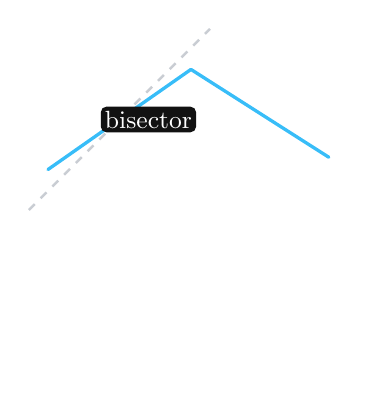
\begin{tikzpicture}[scale=0.92]
  \def\r{2.1}
  \coordinate (O) at (0,0);
  \coordinate (X) at ({\r*cos(160)},{\r*sin(160)});
  \coordinate (Y) at ({\r*cos(90)},{\r*sin(90)});
  \coordinate (Z) at ({\r*cos(25)},{\r*sin(25)});
  \coordinate (M1) at ($(X)!0.5!(Y)$);
  \draw[base] (O) circle (\r);
  \draw[new] (X)--(Y)--(Z);
  \draw[help] ($(M1)+(-1.25,-1.25)$) -- ($(M1)+(1.25,1.25)$);
  \node[tag] at ($(M1)+(0.4,0)$) {bisector};
\end{tikzpicture}
\end{StepDiagram}

\Step{3} Construct the perpendicular bisector of $YZ$.
\begin{StepDiagram}
\begin{tikzpicture}[scale=0.92]
  \def\r{2.1}
  \coordinate (O) at (0,0);
  \coordinate (X) at ({\r*cos(160)},{\r*sin(160)});
  \coordinate (Y) at ({\r*cos(90)},{\r*sin(90)});
  \coordinate (Z) at ({\r*cos(25)},{\r*sin(25)});
  \coordinate (M1) at ($(X)!0.5!(Y)$);
  \coordinate (M2) at ($(Y)!0.5!(Z)$);
  \draw[base] (O) circle (\r);
  \draw[new] (X)--(Y)--(Z);
  \draw[help] ($(M1)+(-1.25,-1.25)$) -- ($(M1)+(1.25,1.25)$);
  \draw[help] ($(M2)+(-1.25, 1.25)$) -- ($(M2)+(1.25,-1.25)$);
\end{tikzpicture}
\end{StepDiagram}

\Step{4} Their intersection is the centre $O$ of the circle (and hence of the arc).
\begin{StepDiagram}
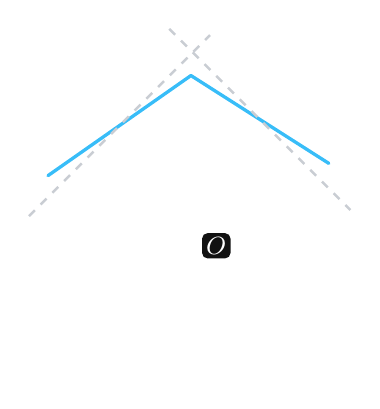
\begin{tikzpicture}[scale=0.92]
  \def\r{2.1}
  \coordinate (O) at (0,0);
  \coordinate (X) at ({\r*cos(160)},{\r*sin(160)});
  \coordinate (Y) at ({\r*cos(90)},{\r*sin(90)});
  \coordinate (Z) at ({\r*cos(25)},{\r*sin(25)});
  \coordinate (M1) at ($(X)!0.5!(Y)$);
  \coordinate (M2) at ($(Y)!0.5!(Z)$);
  \draw[base] (O) circle (\r);
  \draw[new] (X)--(Y)--(Z);
  \draw[help] ($(M1)+(-1.25,-1.25)$) -- ($(M1)+(1.25,1.25)$);
  \draw[help] ($(M2)+(-1.25, 1.25)$) -- ($(M2)+(1.25,-1.25)$);
  \node[dot] at (O) {};
  \node[tag] at ($(O)+(0.35,-0.25)$) {$O$};
\end{tikzpicture}
\end{StepDiagram}

\[
\boxed{\text{Centre of arc }XYZ = \text{intersection of perpendicular bisectors of }XY\text{ and }YZ.}
\]
\end{QAPair}

% ============================================================
% Q3
\begin{QAPair}{Question 3}
\textcolor{gold}{\bfseries Question:} Three non-collinear points $A,B,C$ are such that $AB=BC=3$ cm and $\angle B=120^\circ$. Construct a circle passing through $A,B$ and $C$.
\tcblower
\textcolor{green}{\bfseries Answer:}\par

\Step{1} Draw segment $BC=3$ cm.
\begin{StepDiagram}
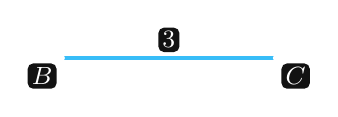
\begin{tikzpicture}[scale=0.92]
  \coordinate (B) at (0,0);
  \coordinate (C) at (3.0,0);
  \draw[new] (B)--(C);
  \node[dot] at (B) {}; \node[tag] at ($(B)+(-0.25,-0.25)$) {$B$};
  \node[dot] at (C) {}; \node[tag] at ($(C)+(0.25,-0.25)$) {$C$};
  \node[tag] at ($(B)!0.5!(C)+(0,0.25)$) {$3$};
\end{tikzpicture}
\end{StepDiagram}

\Step{2} At point $B$, construct an angle of $120^\circ$ and draw the ray.
\begin{StepDiagram}
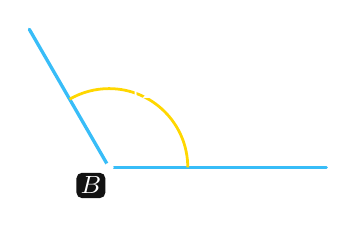
\begin{tikzpicture}[scale=0.92]
  \coordinate (B) at (0,0);
  \coordinate (C) at (3.0,0);
  \coordinate (R) at ({2.2*cos(120)},{2.2*sin(120)});
  \draw[new] (B)--(C);
  \draw[new] (B)--(R);
  \pic[ang,"$120^\circ$",lab,angle radius=10mm,angle eccentricity=1.15] {angle=C--B--R};
  \node[dot] at (B) {}; \node[tag] at ($(B)+(-0.25,-0.25)$) {$B$};
\end{tikzpicture}
\end{StepDiagram}

\Step{3} On this ray, mark point $A$ such that $BA=3$ cm.
\begin{StepDiagram}
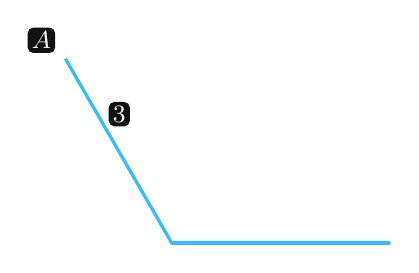
\begin{tikzpicture}[scale=0.92]
  \coordinate (B) at (0,0);
  \coordinate (C) at (3.0,0);
  \coordinate (A) at ({3*cos(120)},{3*sin(120)});
  \draw[new] (B)--(C);
  \draw[new] (B)--(A);
  \node[dot] at (A) {}; \node[tag] at ($(A)+(-0.3,0.2)$) {$A$};
  \node[tag] at ($(B)!0.55!(A)+(0.1,0.35)$) {$3$};
\end{tikzpicture}
\end{StepDiagram}

\Step{4} Join $A$ to $C$ to form $\triangle ABC$.
\begin{StepDiagram}
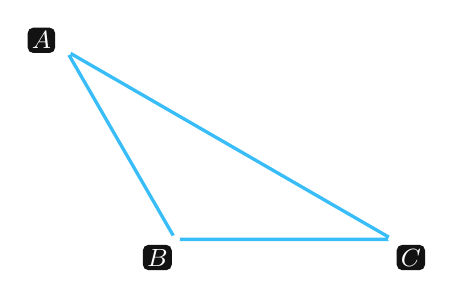
\begin{tikzpicture}[scale=0.92]
  \coordinate (B) at (0,0);
  \coordinate (C) at (3.0,0);
  \coordinate (A) at ({3*cos(120)},{3*sin(120)});
  \draw[new] (A)--(B)--(C)--cycle;
  \node[dot] at (A) {}; \node[tag] at ($(A)+(-0.35,0.15)$) {$A$};
  \node[dot] at (B) {}; \node[tag] at ($(B)+(-0.25,-0.25)$) {$B$};
  \node[dot] at (C) {}; \node[tag] at ($(C)+(0.25,-0.25)$) {$C$};
\end{tikzpicture}
\end{StepDiagram}

\Step{5} Construct perpendicular bisectors of $AB$ and $BC$; they meet at $O$ (circumcentre).
\begin{StepDiagram}
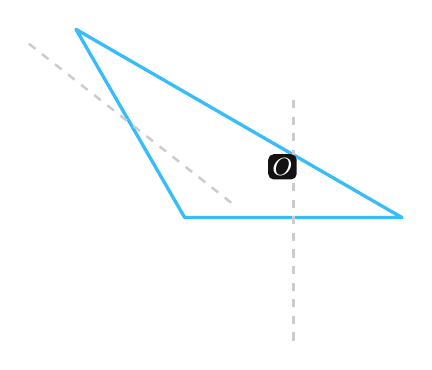
\begin{tikzpicture}[scale=0.92]
  \coordinate (B) at (0,0);
  \coordinate (C) at (3.0,0);
  \coordinate (A) at ({3*cos(120)},{3*sin(120)});
  \coordinate (M1) at ($(A)!0.5!(B)$);
  \coordinate (M2) at ($(B)!0.5!(C)$);
  \draw[new] (A)--(B)--(C)--cycle;
  \draw[help] ($(M1)+(-1.4,1.1)$) -- ($(M1)+(1.4,-1.1)$);
  \draw[help] ($(M2)+(0,-1.7)$) -- ($(M2)+(0,1.7)$);
  \coordinate (O) at (1.0,0.55); % schematic intersection
  \node[dot] at (O) {}; \node[tag] at ($(O)+(0.35,0.15)$) {$O$};
\end{tikzpicture}
\end{StepDiagram}

\Step{6} With centre $O$ and radius $OA$, draw the circle. It passes through $A,B,C$.
\begin{StepDiagram}
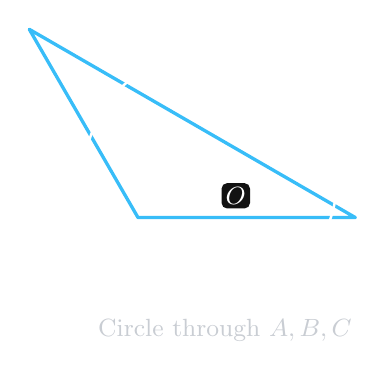
\begin{tikzpicture}[scale=0.92]
  \coordinate (B) at (0,0);
  \coordinate (C) at (3.0,0);
  \coordinate (A) at ({3*cos(120)},{3*sin(120)});
  \coordinate (O) at (1.0,0.55); % schematic
  \draw[new] (A)--(B)--(C)--cycle;
  \draw[base] (O) circle (1.75);
  \node[dot] at (O) {}; \node[tag] at ($(O)+(0.35,-0.25)$) {$O$};
  \node[labm] at (1.2,-1.55) {Circle through $A,B,C$};
\end{tikzpicture}
\end{StepDiagram}

\[
\boxed{\text{Required circle is the circumcircle of }\triangle ABC.}
\]
\end{QAPair}

% ============================================================
% Q4
\begin{QAPair}{Question 4}
\textcolor{gold}{\bfseries Question:} $PQ$ and $QR$ are perpendicular segments such that $PQ=4$ cm and $QR=3$ cm.
Construct a circle passing through $P,Q$ and $R$. What is the radius of that circle?
\tcblower
\textcolor{green}{\bfseries Answer:}\par

\Step{1} Draw $PQ=4$ cm.
\begin{StepDiagram}
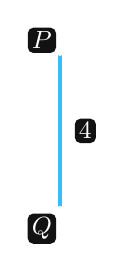
\begin{tikzpicture}[scale=0.92]
  \coordinate (Q) at (0,0);
  \coordinate (P) at (0,2.2);
  \draw[new] (Q)--(P);
  \node[dot] at (P) {}; \node[tag] at ($(P)+(-0.25,0.15)$) {$P$};
  \node[dot] at (Q) {}; \node[tag] at ($(Q)+(-0.25,-0.25)$) {$Q$};
  \node[tag] at ($(Q)!0.5!(P)+(0.35,0)$) {$4$};
\end{tikzpicture}
\end{StepDiagram}

\Step{2} At $Q$, draw a perpendicular to $QP$ and mark $QR=3$ cm.
\begin{StepDiagram}
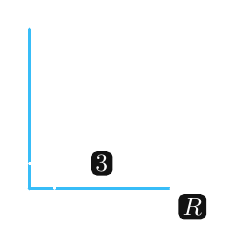
\begin{tikzpicture}[scale=0.92]
  \coordinate (Q) at (0,0);
  \coordinate (P) at (0,2.2);
  \coordinate (R) at (2.0,0);
  \draw[new] (Q)--(P);
  \draw[new] (Q)--(R);
  \draw[base] ($(Q)+(0.35,0)$) -- ($(Q)+(0.35,0.35)$) -- ($(Q)+(0,0.35)$);
  \node[dot] at (R) {}; \node[tag] at ($(R)+(0.25,-0.25)$) {$R$};
  \node[tag] at ($(Q)!0.5!(R)+(0,0.35)$) {$3$};
\end{tikzpicture}
\end{StepDiagram}

\Step{3} Join $P$ to $R$ (this is the hypotenuse).
\begin{StepDiagram}
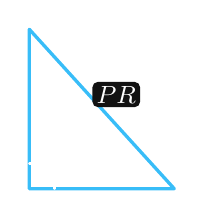
\begin{tikzpicture}[scale=0.92]
  \coordinate (Q) at (0,0);
  \coordinate (P) at (0,2.2);
  \coordinate (R) at (2.0,0);
  \draw[new] (P)--(Q)--(R)--cycle;
  \draw[base] ($(Q)+(0.35,0)$) -- ($(Q)+(0.35,0.35)$) -- ($(Q)+(0,0.35)$);
  \node[tag] at ($(P)!0.5!(R)+(0.2,0.2)$) {$PR$};
\end{tikzpicture}
\end{StepDiagram}

\Step{4} Find midpoint $M$ of $PR$.
\begin{StepDiagram}
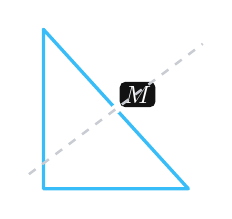
\begin{tikzpicture}[scale=0.92]
  \coordinate (Q) at (0,0);
  \coordinate (P) at (0,2.2);
  \coordinate (R) at (2.0,0);
  \coordinate (M) at ($(P)!0.5!(R)$);
  \draw[new] (P)--(Q)--(R)--cycle;
  \node[dot] at (M) {}; \node[tag] at ($(M)+(0.3,0.2)$) {$M$};
  \draw[help] ($(M)+(-1.2,-0.9)$) -- ($(M)+(1.2,0.9)$);
\end{tikzpicture}
\end{StepDiagram}

\Step{5} With centre $M$ and radius $MP$, draw the circle (passes through $P,Q,R$).
\EqDiagram{Right triangle $\triangle PQR$ at $Q$:\;
$PR=\sqrt{4^2+3^2}=5\text{ cm}$,\;
$\text{radius}=\dfrac{PR}{2}=2.5\text{ cm}$.}
\begin{StepDiagram}
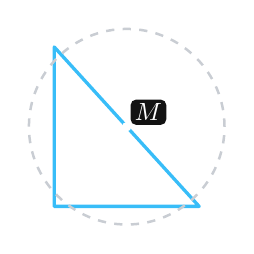
\begin{tikzpicture}[scale=0.92]
  \coordinate (Q) at (0,0);
  \coordinate (P) at (0,2.2);
  \coordinate (R) at (2.0,0);
  \coordinate (M) at ($(P)!0.5!(R)$);
  \draw[new] (P)--(Q)--(R)--cycle;
  \draw[help] (M) circle (1.35);
  \node[dot] at (M) {}; \node[tag] at ($(M)+(0.3,0.2)$) {$M$};
\end{tikzpicture}
\end{StepDiagram}

\[
\boxed{\text{Radius }=2.5\text{ cm}}
\]
\end{QAPair}

% ============================================================
% Q5
\begin{QAPair}{Question 5}
\textcolor{gold}{\bfseries Question:} Draw a circle with the help of any round object, then find its centre.
\tcblower
\textcolor{green}{\bfseries Answer:}\par

\Step{1} Trace the round object to draw the circle.
\begin{StepDiagram}
\MiniCircle{2.1}{
  \node[labm] at (0,-2.55) {Trace a round object};
}
\end{StepDiagram}

\Step{2} Draw a chord $AB$.
\begin{StepDiagram}
\MiniCircle{2.1}{
  \coordinate (A) at (-1.5,0.9);
  \coordinate (B) at ( 1.5,0.9);
  \draw[new] (A)--(B);
  \node[tag] at ($(A)+(-0.25,0.15)$) {$A$};
  \node[tag] at ($(B)+(0.25,0.15)$) {$B$};
}
\end{StepDiagram}

\Step{3} Construct the perpendicular bisector of $AB$.
\begin{StepDiagram}
\MiniCircle{2.1}{
  \coordinate (A) at (-1.5,0.9);
  \coordinate (B) at ( 1.5,0.9);
  \coordinate (M1) at ($(A)!0.5!(B)$);
  \draw[new] (A)--(B);
  \draw[help] ($(M1)+(0,-1.8)$) -- ($(M1)+(0,1.8)$);
}
\end{StepDiagram}

\Step{4} Repeat with another chord; the bisectors meet at the centre $O$.
\begin{StepDiagram}
\MiniCircle{2.1}{
  \coordinate (A) at (-1.5,0.9);
  \coordinate (B) at ( 1.5,0.9);
  \coordinate (C) at (-1.1,-0.4);
  \coordinate (D) at ( 1.1,1.6);
  \coordinate (M1) at ($(A)!0.5!(B)$);
  \coordinate (M2) at ($(C)!0.5!(D)$);
  \draw[new] (A)--(B);
  \draw[new] (C)--(D);
  \draw[help] ($(M1)+(0,-1.8)$) -- ($(M1)+(0,1.8)$);
  \draw[help] ($(M2)+(-1.8,0)$) -- ($(M2)+(1.8,0)$);
  \node[dot] at (O) {}; \node[tag] at ($(O)+(0.35,-0.25)$) {$O$};
}
\end{StepDiagram}

\[
\boxed{\text{Centre }= \text{intersection of perpendicular bisectors of two chords.}}
\]
\end{QAPair}

% ============================================================
% Q6
\begin{QAPair}{Question 6}
\textcolor{gold}{\bfseries Question:} Find the centre of an arc $DEF$ such that chord $DE=3.5$ cm, chord $EF=4.2$ cm
and the angle between both segments is $60^\circ$.
\tcblower
\textcolor{green}{\bfseries Answer:}\par

\Step{1} Draw $DE=3.5$ cm.
\begin{StepDiagram}

\begin{tikzpicture}[scale=0.92]
  \coordinate (D) at (-2.4,0);
  \coordinate (E) at (0,0);
  \draw[new] (D)--(E);
  \node[dot] at (D) {}; \node[tag] at ($(D)+(-0.25,-0.25)$) {$D$};
  \node[dot] at (E) {}; \node[tag] at ($(E)+(0.25,-0.25)$) {$E$};
  \node[tag] at ($(D)!0.5!(E)+(0,0.35)$) {$3.5$};
\end{tikzpicture}
\end{StepDiagram}

\Step{2} At $E$, construct $\angle DEF=60^\circ$.
\begin{StepDiagram}
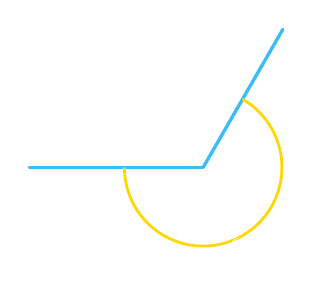
\begin{tikzpicture}[scale=0.92]
  \coordinate (D) at (-2.4,0);
  \coordinate (E) at (0,0);
  \coordinate (Ray) at ({2.2*cos(60)},{2.2*sin(60)});
  \draw[new] (D)--(E);
  \draw[new] (E)--(Ray);
  \pic[ang,"$60^\circ$",lab,angle radius=10mm,angle eccentricity=1.15] {angle=D--E--Ray};
\end{tikzpicture}
\end{StepDiagram}

\Step{3} On the second arm, mark $F$ such that $EF=4.2$ cm.
\begin{StepDiagram}
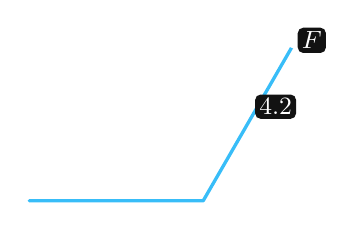
\begin{tikzpicture}[scale=0.92]
  \coordinate (D) at (-2.4,0);
  \coordinate (E) at (0,0);
  \coordinate (F) at ({2.5*cos(60)},{2.5*sin(60)});
  \draw[new] (D)--(E)--(F);
  \node[dot] at (F) {}; \node[tag] at ($(F)+(0.25,0.05)$) {$F$};
  \node[tag] at ($(E)!0.6!(F)+(0.25,0.0)$) {$4.2$};
\end{tikzpicture}
\end{StepDiagram}

\Step{4} Join $D$ to $F$ to form $\triangle DEF$.
\begin{StepDiagram}
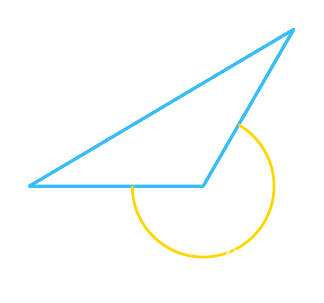
\begin{tikzpicture}[scale=0.92]
  \coordinate (D) at (-2.4,0);
  \coordinate (E) at (0,0);
  \coordinate (F) at ({2.5*cos(60)},{2.5*sin(60)});
  \draw[new] (D)--(E)--(F);
  \draw[new] (D)--(F);
  \pic[ang,"$60^\circ$",lab,angle radius=9mm,angle eccentricity=1.15] {angle=D--E--F};
\end{tikzpicture}
\end{StepDiagram}

\Step{5} Construct perpendicular bisectors of $DE$ and $EF$; their intersection is $O$.
\begin{StepDiagram}
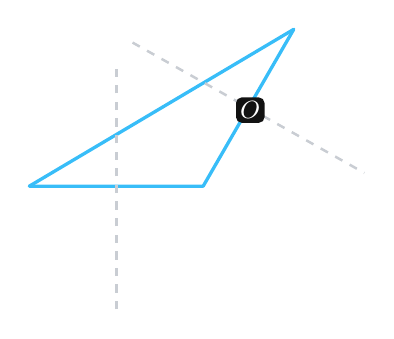
\begin{tikzpicture}[scale=0.92]
  \coordinate (D) at (-2.4,0);
  \coordinate (E) at (0,0);
  \coordinate (F) at ({2.5*cos(60)},{2.5*sin(60)});
  \coordinate (M1) at ($(D)!0.5!(E)$);
  \coordinate (M2) at ($(E)!0.5!(F)$);
  \draw[new] (D)--(E)--(F);
  \draw[new] (D)--(F);
  \draw[help] ($(M1)+(0,-1.7)$) -- ($(M1)+(0,1.7)$);
  \draw[help] ($(M2)+(-1.6,0.9)$) -- ($(M2)+(1.6,-0.9)$);
  \coordinate (O) at (0.3,0.9); % schematic
  \node[dot] at (O) {}; \node[tag] at ($(O)+(0.35,0.15)$) {$O$};
\end{tikzpicture}
\end{StepDiagram}

\Step{6} With centre $O$ and radius $OE$, draw the circle; the arc $DEF$ is part of this circle.
\begin{StepDiagram}
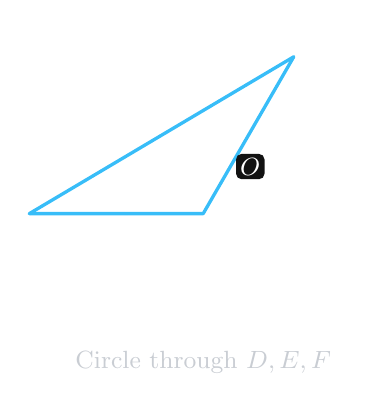
\begin{tikzpicture}[scale=0.92]
  \coordinate (D) at (-2.4,0);
  \coordinate (E) at (0,0);
  \coordinate (F) at ({2.5*cos(60)},{2.5*sin(60)});
  \coordinate (O) at (0.3,0.9); % schematic
  \draw[base] (O) circle (1.65);
  \draw[new] (D)--(E)--(F);
  \draw[new] (D)--(F);
  \node[dot] at (O) {}; \node[tag] at ($(O)+(0.35,-0.25)$) {$O$};
  \node[labm] at (0,-2.05) {Circle through $D,E,F$};
\end{tikzpicture}
\end{StepDiagram}

\[
\boxed{\text{Centre of arc }DEF = \text{circumcentre of }\triangle DEF.}
\]
\end{QAPair}

% ============================================================
% Q7
\begin{QAPair}{Question 7}
\textcolor{gold}{\bfseries Question:} Draw an arc of any length. Complete the circle without finding its centre, of which the given arc is the part.
\tcblower
\textcolor{green}{\bfseries Answer:}\par

\Step{1} While drawing the arc, you used a compass (fixed opening).
\begin{StepDiagram}
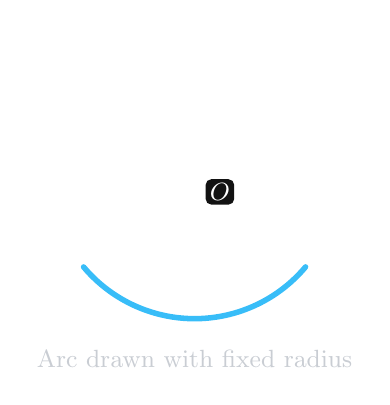
\begin{tikzpicture}[scale=0.92]
  \def\r{2.0}
  \coordinate (O) at (0,0);
  \draw[base] (O) circle (\r);
  \draw[new, line width=2pt] ({\r*cos(220)},{\r*sin(220)}) arc (220:320:\r);
  \node[dot] at (O) {}; \node[tag] at ($(O)+(0.35,-0.25)$) {$O$};
  \node[labm] at (0,-2.55) {Arc drawn with fixed radius};
\end{tikzpicture}
\end{StepDiagram}

\Step{2} Keep the \textbf{same compass opening} (same radius).
\begin{StepDiagram}
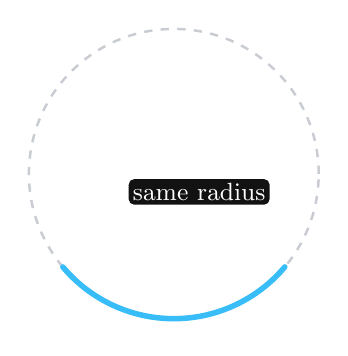
\begin{tikzpicture}[scale=0.92]
  \def\r{2.0}
  \coordinate (O) at (0,0);
  \draw[help] (O) circle (\r);
  \draw[new, line width=2pt] ({\r*cos(220)},{\r*sin(220)}) arc (220:320:\r);
  \node[dot] at (O) {}; \node[tag] at ($(O)+(0.35,-0.25)$) {same radius};
\end{tikzpicture}
\end{StepDiagram}

\Step{3} Rotate the compass and draw the remaining part to complete the circle.
\begin{StepDiagram}
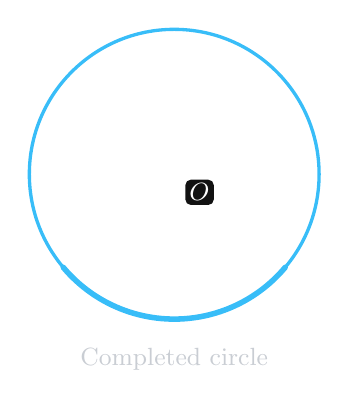
\begin{tikzpicture}[scale=0.92]
  \def\r{2.0}
  \coordinate (O) at (0,0);
  \draw[new] (O) circle (\r);
  \draw[new, line width=2pt] ({\r*cos(220)},{\r*sin(220)}) arc (220:320:\r);
  \node[dot] at (O) {}; \node[tag] at ($(O)+(0.35,-0.25)$) {$O$};
  \node[labm] at (0,-2.55) {Completed circle};
\end{tikzpicture}
\end{StepDiagram}

\[
\boxed{\text{Use the same compass radius used to draw the arc; continue to complete the circle.}}
\]
\end{QAPair}

% ============================================================
% Q8
\begin{QAPair}{Question 8}
\textcolor{gold}{\bfseries Question:} An engineer is constructing a circular path in a recreational park as shown.
He wants to plant a pine tree in the centre of the circular path.
(i) How will he locate the centre of the path? \quad (ii) What is the radius of the circular path?
\tcblower
\textcolor{green}{\bfseries Answer:}\par

\Step{1} Choose two different chords on the boundary of the path.
\begin{StepDiagram}
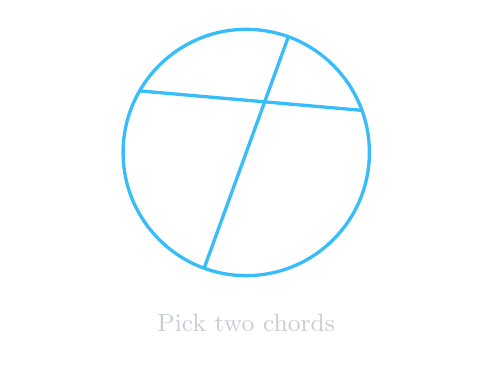
\begin{tikzpicture}[scale=0.92]
  \def\r{1.7}
  \coordinate (O) at (0,0);
  \draw[base] (-3,-1.7) rectangle (3,1.7);
  \draw[new] (O) circle (\r);
  \coordinate (A) at ({\r*cos(150)},{\r*sin(150)});
  \coordinate (B) at ({\r*cos(20)},{\r*sin(20)});
  \coordinate (C) at ({\r*cos(250)},{\r*sin(250)});
  \coordinate (D) at ({\r*cos(70)},{\r*sin(70)});
  \draw[new] (A)--(B);
  \draw[new] (C)--(D);
  \node[labm] at (0,-2.35) {Pick two chords};
\end{tikzpicture}
\end{StepDiagram}

\Step{2} Draw a line perpendicular to each chord at its midpoint (perpendicular bisectors).
\begin{StepDiagram}
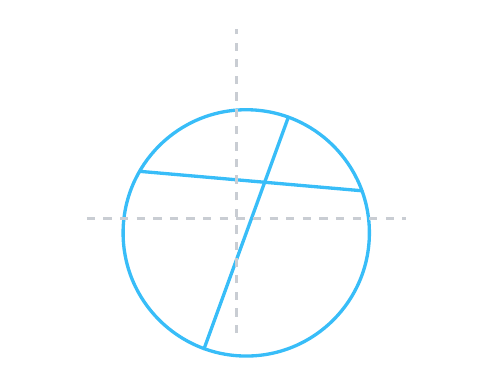
\begin{tikzpicture}[scale=0.92]
  \def\r{1.7}
  \coordinate (O) at (0,0);
  \draw[base] (-3,-1.7) rectangle (3,1.7);
  \draw[new] (O) circle (\r);
  \coordinate (A) at ({\r*cos(150)},{\r*sin(150)});
  \coordinate (B) at ({\r*cos(20)},{\r*sin(20)});
  \coordinate (C) at ({\r*cos(250)},{\r*sin(250)});
  \coordinate (D) at ({\r*cos(70)},{\r*sin(70)});
  \coordinate (M1) at ($(A)!0.5!(B)$);
  \coordinate (M2) at ($(C)!0.5!(D)$);
  \draw[new] (A)--(B);
  \draw[new] (C)--(D);
  \draw[help] ($(M1)+(-0.2,-2.1)$) -- ($(M1)+(-0.2,2.1)$);
  \draw[help] ($(M2)+(-2.2,0.2)$) -- ($(M2)+( 2.2,0.2)$);
\end{tikzpicture}
\end{StepDiagram}

\Step{3} The two perpendicular bisectors intersect at the centre (plant the tree there).
\begin{StepDiagram}
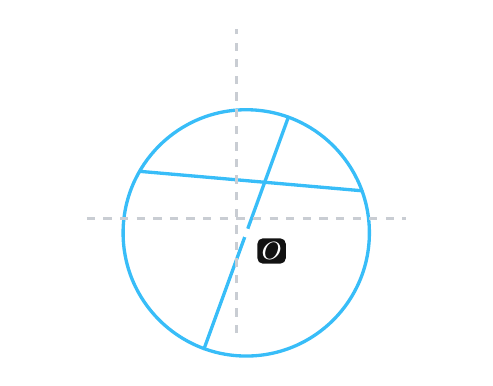
\begin{tikzpicture}[scale=0.92]
  \def\r{1.7}
  \coordinate (O) at (0,0);
  \draw[base] (-3,-1.7) rectangle (3,1.7);
  \draw[new] (O) circle (\r);
  \coordinate (A) at ({\r*cos(150)},{\r*sin(150)});
  \coordinate (B) at ({\r*cos(20)},{\r*sin(20)});
  \coordinate (C) at ({\r*cos(250)},{\r*sin(250)});
  \coordinate (D) at ({\r*cos(70)},{\r*sin(70)});
  \coordinate (M1) at ($(A)!0.5!(B)$);
  \coordinate (M2) at ($(C)!0.5!(D)$);
  \draw[new] (A)--(B);
  \draw[new] (C)--(D);
  \draw[help] ($(M1)+(-0.2,-2.1)$) -- ($(M1)+(-0.2,2.1)$);
  \draw[help] ($(M2)+(-2.2,0.2)$) -- ($(M2)+( 2.2,0.2)$);
  \node[dot] at (O) {}; \node[tag] at ($(O)+(0.35,-0.25)$) {$O$};
\end{tikzpicture}
\end{StepDiagram}

\Step{4} From the figure, the shown $50$ m is a diameter, so $r=\dfrac{50}{2}=25$ m.
\begin{StepDiagram}
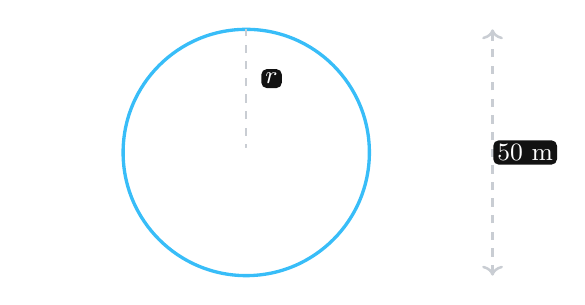
\begin{tikzpicture}[scale=0.92]
  \def\r{1.7}
  \coordinate (O) at (0,0);
  \draw[base] (-3,-1.7) rectangle (3,1.7);
  \draw[new] (O) circle (\r);
  \draw[help,<->] (3.4,-1.7) -- (3.4,1.7);
  \node[tag] at (3.85,0) {$50\text{ m}$};
  \draw[help] (O)--(0,\r);
  \node[tag] at ($(O)!0.6!(0,\r)+(0.35,0)$) {$r$};
  \node[dot] at (O) {};
\end{tikzpicture}
\end{StepDiagram}

\[
\boxed{\text{Centre: intersection of perpendicular bisectors of two chords, }\quad r=25\text{ m}.}
\]
\end{QAPair}

% ============================================================
% Q9
\begin{QAPair}{Question 9}
\textcolor{gold}{\bfseries Question:} A factory produces arc-shaped tiles of inner radius $7$ inches.
Arc length of each tile is $2$ inches. How many tiles are required to make a complete circular design?
\tcblower
\textcolor{green}{\bfseries Answer:}\par

\Step{1} Circumference of radius $7$ is $C=2\pi r=14\pi$ inches.
\begin{StepDiagram}
\begin{tikzpicture}[scale=0.92]
  \def\r{2.0}
  \coordinate (O) at (0,0);
  \draw[base] (O) circle (\r);
  \draw[help] (O)--(\r,0);
  \node[tag] at ($(O)!0.6!(\r,0)+(0,0.25)$) {$r=7$};
  \node[labm] at (0,-2.55) {$C=2\pi r$};
\end{tikzpicture}
\end{StepDiagram}

\Step{2} Each tile covers $2$ inches, so $N=\dfrac{C}{2}=\dfrac{14\pi}{2}=7\pi$.
\begin{StepDiagram}
\begin{tikzpicture}[scale=0.92]
  \def\r{2.0}
  \coordinate (O) at (0,0);
  \draw[base] (O) circle (\r);
  \draw[new, line width=2pt] ({\r*cos(10)},{\r*sin(10)}) arc (10:40:\r);
  \node[tag] at ({1.5*cos(25)},{1.5*sin(25)}) {$2$ in};
  \node[labm] at (0,-2.55) {$N=\dfrac{C}{2}$};
\end{tikzpicture}
\end{StepDiagram}

\Step{3} Round up to a whole tile: $7\pi\approx 21.99 \Rightarrow 22$ tiles.
\EqDiagram{$N=7\pi\approx 21.99\;\Rightarrow\;\boxed{22\ \text{tiles}}$}

\[
\boxed{22\ \text{tiles}}
\]
\end{QAPair}

% ============================================================
% Q10
\begin{QAPair}{Question 10}
\textcolor{gold}{\bfseries Question:} In the figure a boat swing is shown. Trace the circular path of swing during a complete round.
\tcblower
\textcolor{green}{\bfseries Answer:}\par

\Step{1} Identify the pivot point $O$ (the hanging point).
\begin{StepDiagram}
\begin{tikzpicture}[scale=0.92]
  \coordinate (O) at (0,2.0);
  \draw[base] (-1.7,0) -- (0,2.0) -- (1.7,0);
  \node[dot] at (O) {}; \node[tag] at ($(O)+(0.35,0.15)$) {$O$};
  \node[labm] at (0,-0.7) {Pivot point};
\end{tikzpicture}
\end{StepDiagram}

\Step{2} Measure the rope/arm length $OS$ (this is the radius).
\begin{StepDiagram}
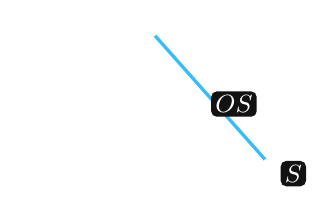
\begin{tikzpicture}[scale=0.92]
  \coordinate (O) at (0,2.0);
  \coordinate (S) at (1.6,0.2);
  \draw[base] (-1.7,0) -- (0,2.0) -- (1.7,0);
  \draw[new] (O)--(S);
  \node[dot] at (O) {};
  \node[dot] at (S) {};
  \node[tag] at ($(O)!0.55!(S)+(0.25,0)$) {$OS$};
  \node[tag] at ($(S)+(0.35,-0.15)$) {$S$};
\end{tikzpicture}
\end{StepDiagram}

\Step{3} With centre $O$ and radius $OS$, draw the circular path.
\begin{StepDiagram}
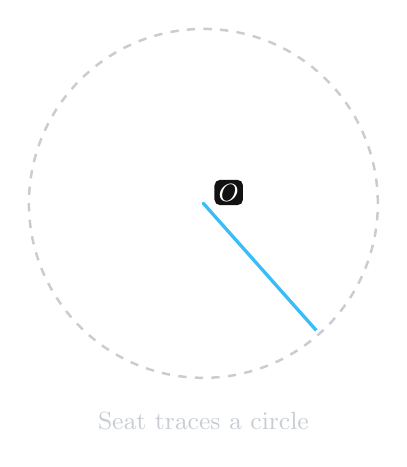
\begin{tikzpicture}[scale=0.92]
  \coordinate (O) at (0,2.0);
  \coordinate (S) at (1.6,0.2);
  \draw[base] (-2.3,0) -- (2.3,0);
  \draw[base] (-1.7,0) -- (0,2.0) -- (1.7,0);
  \node[dot] at (O) {}; \node[tag] at ($(O)+(0.35,0.15)$) {$O$};
  \draw[new] (O)--(S);
  \node[dot] at (S) {};
  \pgfmathsetmacro{\rad}{sqrt((1.6)^2 + (1.8)^2)}
  \draw[help] (O) circle (\rad);
  \node[labm] at (0,-1.0) {Seat traces a circle};
\end{tikzpicture}
\end{StepDiagram}

\[
\boxed{\text{The swing seat moves on a circle with centre at the pivot point.}}
\]
\end{QAPair}

\end{document}
